% https://manualdelatex.com/tutoriales/figuras

% standar 
\begin{figure}
\includegraphics[opciones]{imagen}
\end{figure}

% Imagen centrada y de tamaño%50
\begin{figure}[htb]
   \centering
    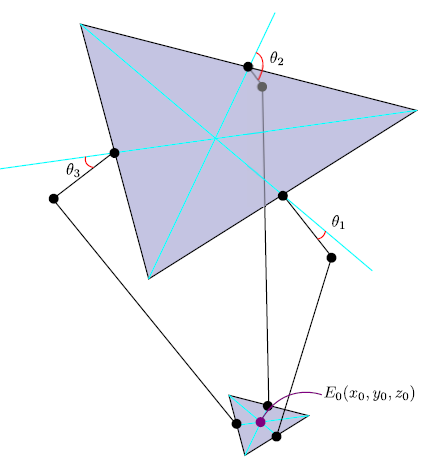
\includegraphics[width=0.5\linewidth]{Main/Chapter4/Metodo_A_Modelacion_Cinematica_Posicion_1.png}
    \caption{Fotografía de un paraguas}
    %\label{f:Metodo_A_Modelacion_Cinematica_Posicion_1}
\end{figure}

% Multiples imagenes        
\usepackage{subfig}
\begin{figure}
 \centering
  \subfloat[Gatito]{
   %\label{f:gato}
    \includegraphics[width=0.3\textwidth]{gato.png}}
  \subfloat[Tigre]{
   %\label{f:tigre}
    \includegraphics[width=0.3\textwidth]{tigre.png}}
  \subfloat[Conejo]{
   %\label{f:conejo}
    \includegraphics[width=0.3\textwidth]{conejo.png}}
 \caption{Múltiples imágenes}
 %\label{f:animales}
\end{figure}

\begin{figure}[!tbp]
  \begin{subfigure}[b]{0.49\textwidth}
    \includegraphics[width=\textwidth, height=\textwidth]{img1.jpg}
    \caption{Primera imagen.}
    \label{fig:f1}
  \end{subfigure}
  \hfill
  \begin{subfigure}[b]{0.49\textwidth}
    \includegraphics[width=\textwidth, height=\textwidth]{img2.jpg}
    \caption{Segunda imagen.}
    \label{fig:f2}
  \end{subfigure}
  \caption{Dos imágenes en la misma figura.}
\end{figure}
 
